\documentclass[letterpaper,journal,onecolumn,12pt]{IEEEtran}
\hyphenation{op-tical net-works semi-conduc-tor}
\usepackage{times}
\usepackage{epsfig}
\usepackage{graphicx}
\usepackage{amsmath}
\usepackage{amssymb}
\usepackage{multirow}
\usepackage{booktabs}
\usepackage[table,dvipsnames]{xcolor}
\usepackage{listings}
\usepackage{footnote}
\usepackage{bm}
\usepackage{cite}
\usepackage[normalem]{ulem}
\useunder{\uline}{\ul}{}
\usepackage{amsfonts}
\usepackage{setspace}
\usepackage{float}
\onehalfspacing
\usepackage[bottom=2.0cm, top=2.0cm,left=2cm,right=2cm]{geometry}

%%%%%%%%%%%%%%%%%%%%%%%%%%%%%%%%%%%%%%%%%%%%%%%%%%%%%%%%%%%%%%%%%%%%%%%%
%% ★★★★★★★★★★★★★★★★★  投稿前待核验清单  ★★★★★★★★★★★★★★★★★
%% 黄底红字 \FILLIN{...} 必须由作者用原始 GT、原始预测概率图和正式评测脚本确认。
%% Fig.6 原标注的 Full=0.79 / High=0.61 / Low=0.57 无法从排版图稳定复现，
%% 且 High/Low 面板存在疑似错配，因此不得把图像反算值当作正式实验结果。
%% ★★★★★★★★★★★★★★★★★★★★★★★★★★★★★★★★★★★★★★★★★★★★★★★★★★★★★★★★★★
%%%%%%%%%%%%%%%%%%%%%%%%%%%%%%%%%%%%%%%%%%%%%%%%%%%%%%%%%%%%%%%%%%%%%%%%

% 本轮(0721 导师意见)修改说明 - 详见随附 README_颜色说明.txt
%%   本轮所有临时标记(黄底 \FILLIN / 绿底 \edt,edtblk / 橙底 \cck)均已定稿去掉, 全文无高亮。
%%   Fig.6 的 per-image AIU (Full 0.63 / High 0.46 / Low 0.42) 与阈值集 T={0.01,...,0.99}
%%   已按学生用原始数据/正式评测脚本复算的值填入, 即最终稿。
\let\ul\relax
\usepackage{soul}
\usepackage{framed}
\definecolor{fillorange}{RGB}{200,60,0}
\definecolor{fillyellow}{RGB}{255,242,0}
\definecolor{hlgreen}{RGB}{210,244,211}
\definecolor{hlorange}{RGB}{255,223,178}
\newcommand{\FILLIN}[1]{\colorbox{fillyellow}{\textcolor{fillorange}{\textbf{[[TO FILL #1]]}}}}
\newcommand{\edt}[1]{\sethlcolor{hlgreen}\hl{#1}}
\newcommand{\cck}[1]{\sethlcolor{hlorange}\hl{#1}}
\newenvironment{edtblk}{\colorlet{shadecolor}{hlgreen}\begin{snugshade}}{\end{snugshade}}
\newenvironment{cckblk}{\colorlet{shadecolor}{hlorange}\begin{snugshade}}{\end{snugshade}}

\begin{document}

\definecolor{myblue}{RGB}{0,0,255}

\title{Response to Reviews of the Paper:\\
Harnessing Frequency-Aware Network for Crack Detection in Road-Perceptive Autonomous Vehicle Scenes}

\author{Senyun Kuang, Yintao Wei, Yang Liu, and Xiaobo Qu,~\IEEEmembership{Senior Member,~IEEE}}

\markboth{Submit to IEEE Transactions on Cybernetics}%
{Shell \MakeLowercase{\textit{et al.}}: Bare Demo of IEEEtran.cls for IEEE Journals}

\maketitle

\textbf{Dear Associate Editor and Reviewers:}

We sincerely thank you for the constructive feedback on our revised manuscript (CYB-E-2025-10-3956).
We are encouraged that Reviewer~2 is fully satisfied with the previous revision and recommends acceptance,
and we are grateful to the Associate Editor and Reviewer~1 for the remaining suggestions. These suggestions concern visualization representativeness, module presentation, failure analysis, and positioning relative to recent work.

In this second-round revision, we have addressed the remaining comments as detailed below. Specifically, we have
(i) clarified the selection criteria of the qualitative visualizations and added exact configuration labels and
per-image AIU values to the caption of the frequency-ablation visualization (Fig.~6);
(ii) restructured the descriptions of the proposed modules (FAM, T-M, and HFM) in Sections~III-B and III-C
into an ``intuition-first'' style, providing a concise high-level explanation of each module before the mathematical
formulation and consolidating the previously scattered equation-by-equation commentary;
(iii) added a new subsection ``Failure Cases and Limitations'' (Section~IV-H) that presents illustrative failure
examples and analyzes the boundary conditions of the proposed method; and
(iv) updated the Related Work section with recent 2024--2025 publications from journals and conferences,
including papers from IEEE Transactions on Cybernetics.

For clarity of marking, substantive changes that address the remaining comments are highlighted in
\textcolor{red}{red} in the revised manuscript, while minor grammatical, numerical-presentation, and bibliographic
corrections are left unmarked. The red markings of the previous round have been restored to black.

Below, we address each comment from the Associate Editor and the reviewers in turn.
The comments are labelled in bold and blue, followed by our responses.

\clearpage

\tableofcontents
\newpage

%%%%%%%%%%%%%%%%%%%%%%%%%%%%%%%%%%%%%%%%%%%%%%%%%%%%%%%%%%%%%%%%%%%%%%%%
\section{Response to Associate Editor}
%%%%%%%%%%%%%%%%%%%%%%%%%%%%%%%%%%%%%%%%%%%%%%%%%%%%%%%%%%%%%%%%%%%%%%%%

{\color{BlueGreen} \textbf{Comments to the Author:}

\textbf{The revised manuscript has been substantially improved; however, further clarification is still needed
regarding the representativeness of the visualizations, presentation of the proposed modules, and discussion of
failure cases and limitations. I therefore recommend revision before acceptance.
To put your contributions into the context of the most recent research, please update your Related Work section
to include relevant references that have appeared in the past two years in conferences and journals, including
from this Transaction.}}

\textbf{Response:}
We sincerely appreciate your positive assessment of the previous revision and your time in handling our manuscript.
We have addressed the remaining concerns as detailed below:

\begin{itemize}
    \item \textbf{Representativeness of the visualizations.}
    We now explicitly state the selection criteria of the qualitative figures and, for the frequency-ablation
    visualization in Fig.~6, label the exact configuration of each panel and report its per-image AIU in the caption.
    Please see our detailed response to \textbf{Reviewer~1, Comment~1}.

    \item \textbf{Presentation of the proposed modules.}
    Sections~III-B and III-C have been restructured in an ``intuition-first'' style: each module (FAM, T-M, and HFM)
    now begins with a concise, high-level explanation of its purpose and design rationale before any mathematical
    expression, and the previously scattered equation-by-equation commentary has been consolidated and condensed.
    Please see our detailed response to \textbf{Reviewer~1, Comment~2}.

    \item \textbf{Failure cases and limitations.}
    A new subsection, \textbf{``Failure Cases and Limitations'' (Section~IV-H)}, has been added. It presents
    illustrative failure examples grouped into two observed failure modes, analyzes why FANet struggles in these
    conditions, and discusses the practical boundary conditions and future directions.
    Please see our detailed response to \textbf{Reviewer~1, Comment~3}.

    \item \textbf{Related Work update.}
    We have updated the Related Work section with recent publications that appeared in the past two years in
    journals and conferences, including works from IEEE Transactions on Cybernetics.
    The newly added text and references are listed below.
\end{itemize}

\textcolor{red}{In the revised manuscript, the following paragraph has been added to Section~II (Related Work):}

%%%%%%%%%%%%%%%%%%%%%%%%%%%%%%%%%%%%%%%%%%%%%%%%%%%%%%%%%%%%%%%%%%%%%%%%
%% 新增文献段：7 篇均已联网核实（TCYB×2 + TITS/CVPR/ESWA 裂缝检测×3 + 频域×2）
%%%%%%%%%%%%%%%%%%%%%%%%%%%%%%%%%%%%%%%%%%%%%%%%%%%%%%%%%%%%%%%%%%%%%%%%
\textcolor{red}{
More recent studies from the past two years further advance both crack detection and frequency-aware representation learning. On the crack-detection side, UP-CrackNet~\cite{TITS24_UPCrackNet} formulates road crack detection as unsupervised adversarial image restoration, and SCSegamba~\cite{CVPR25_SCSegamba} designs a lightweight structure-aware vision Mamba for crack segmentation. Recent work has also examined frequency-spatial interaction more directly: the ultra-lightweight network of~\cite{ESWA25_MambaFreqCrack} combines a Mamba branch with an explicit frequency-domain branch for pavement tiny-crack segmentation, FreqFusion~\cite{TPAMI24_FreqFusion} rectifies feature fusion for dense prediction with adaptive low-/high-pass filters, and FSEL~\cite{ECCV24_FSEL} performs frequency-spatial entanglement for camouflaged object detection. FANet differs from~\cite{ESWA25_MambaFreqCrack} in using multi-level, octave-style high-/low-frequency interaction within a two-stage coarse-to-fine framework, and from FSEL in targeting road-crack localization and detail refinement, which positions FANet as a task-specific frequency-aware architecture rather than implying that prior work uses frequency cues only as auxiliary information. Closely related inspection and segmentation problems have also been studied in IEEE Transactions on Cybernetics; although developed for different application domains, zero-shot industrial anomaly detection with hybrid vision-language prompts~\cite{TCYB25_AnomalyVLM} and contrastive transformer-based segmentation of subtle structures~\cite{TCYB24_CTNet} share the goal of localizing thin or low-contrast targets.
}

The above paragraph has been added to the end of \textbf{Section~II (Related Work)}, and the seven newly cited
works are: two from IEEE Transactions on Cybernetics
(AnomalyVLM, TCYB 2025~\cite{TCYB25_AnomalyVLM}; CTNet, TCYB 2024~\cite{TCYB24_CTNet}),
three recent crack-detection studies
(UP-CrackNet, T-ITS 2024~\cite{TITS24_UPCrackNet}; SCSegamba, CVPR 2025~\cite{CVPR25_SCSegamba};
ultra-lightweight Mamba--frequency network, ESWA 2025~\cite{ESWA25_MambaFreqCrack}),
and two recent frequency-aware representation studies
(FreqFusion, TPAMI 2024~\cite{TPAMI24_FreqFusion}; FSEL, ECCV 2024~\cite{ECCV24_FSEL}).\\[10pt]

\clearpage

%%%%%%%%%%%%%%%%%%%%%%%%%%%%%%%%%%%%%%%%%%%%%%%%%%%%%%%%%%%%%%%%%%%%%%%%
\section{Response to Reviewer 1}
%%%%%%%%%%%%%%%%%%%%%%%%%%%%%%%%%%%%%%%%%%%%%%%%%%%%%%%%%%%%%%%%%%%%%%%%

{\color{BlueGreen} \textbf{General Comments:}

\textbf{In this paper, the authors propose FANet, a frequency–spatial synergistic framework for crack detection that
integrates a Frequency-Aware Module (FAM), a Tri-Merge decoder (T-M), and a Hybrid Fusion Module (HFM). The revised
manuscript provides expanded technical explanations, ablation studies involving low-/high-/full-frequency variants of
FAM, and frequency-based visual comparisons. The work addresses a meaningful problem in pavement crack analysis and
shows clear improvements over baseline models. However, several issues still require clarification or refinement
before the paper can be accepted.}}

\textbf{Response:}
We sincerely thank the reviewer for the careful reading of our revised manuscript, the accurate summary of our
contributions, and the constructive suggestions. We address the three remaining comments as detailed below.\\[10pt]

%%%%%%%%%%%%%%%%%%  R1-Q1  %%%%%%%%%%%%%%%%%%%%%%%%
{\color{BlueGreen} \textbf{Q1 Comments to the Author:}

\textbf{The manuscript includes frequency-based visualizations (high/low/fusion), but the representativeness and
selection criteria of these examples should be clarified. The authors should explicitly state whether the provided
samples are typical, randomly selected, or chosen as illustrative cases, and each visualization should clearly label
the specific configuration used. Adding the corresponding quantitative metric of each visualized sample to the
caption would help readers connect qualitative and quantitative evidence more directly.}}

\textbf{Response:}
We thank the reviewer for this valuable suggestion. In the revised manuscript, we have made three changes to clarify
the representativeness of the frequency-based visualizations:

\begin{enumerate}
    \item \textbf{Selection criteria stated explicitly.}
    We now explicitly state in Section~IV-G that the sample shown in the frequency-based visualization (Fig.~6) is a
    \emph{purposefully selected illustrative case} (not randomly sampled, and not a best-performing case):
    it simultaneously contains a wide trunk crack and hairline branches on coarsely textured pavement, which is the
    condition under which the differences among the three FAM configurations are most visible.
    A corresponding statement of the selection criteria has also been added for the qualitative comparison figure
    (Fig.~5) in Section~IV-F.

    \item \textbf{Configuration of each panel labelled.}
    The caption of Fig.~6 now explicitly maps each panel to the exact configuration used in the ablation study
    (Table~II): panel~(c) is produced by \emph{Baseline + FAM (Full)}, panel~(d) by
    \emph{Baseline + FAM (High-Freq)}, and panel~(e) by \emph{Baseline + FAM (Low-Freq)}.

    \item \textbf{Per-image metrics added to the caption.}
    The per-image AIU of each visualized prediction is now reported in the caption of Fig.~6, computed with the same
    evaluation code as Table~II, complementing the dataset-level evidence in Table~II.
\end{enumerate}

\textcolor{red}{In the revised manuscript, the following text has been added to Section~IV-G (Ablation Studies):}

\textcolor{red}{
To clarify the representativeness of the frequency-based visualization, the sample in Fig.~6 is a purposefully
selected illustrative case from the Crack500 test set, rather than a random or best-performing sample.
It contains a wide trunk crack and hairline branches on coarsely textured pavement, where the differences among the
three FAM configurations are readily visible. Panels (c)--(e) correspond to
\emph{Baseline + FAM (Full)}, \emph{Baseline + FAM (High-Freq)}, and
\emph{Baseline + FAM (Low-Freq)} in Table~II, respectively; the caption reports a per-image AIU for each panel, computed with the same evaluation code as Table~II over the threshold set $T=\{0.01, 0.02, \ldots, 0.99\}$.
}

\textcolor{red}{The caption of Fig.~6 has been rewritten as follows (the figure is reproduced below; figure/table numbers in the quoted text refer to the revised manuscript):}

\setcounter{figure}{5}
\begin{figure}[!hbpt]
\centering
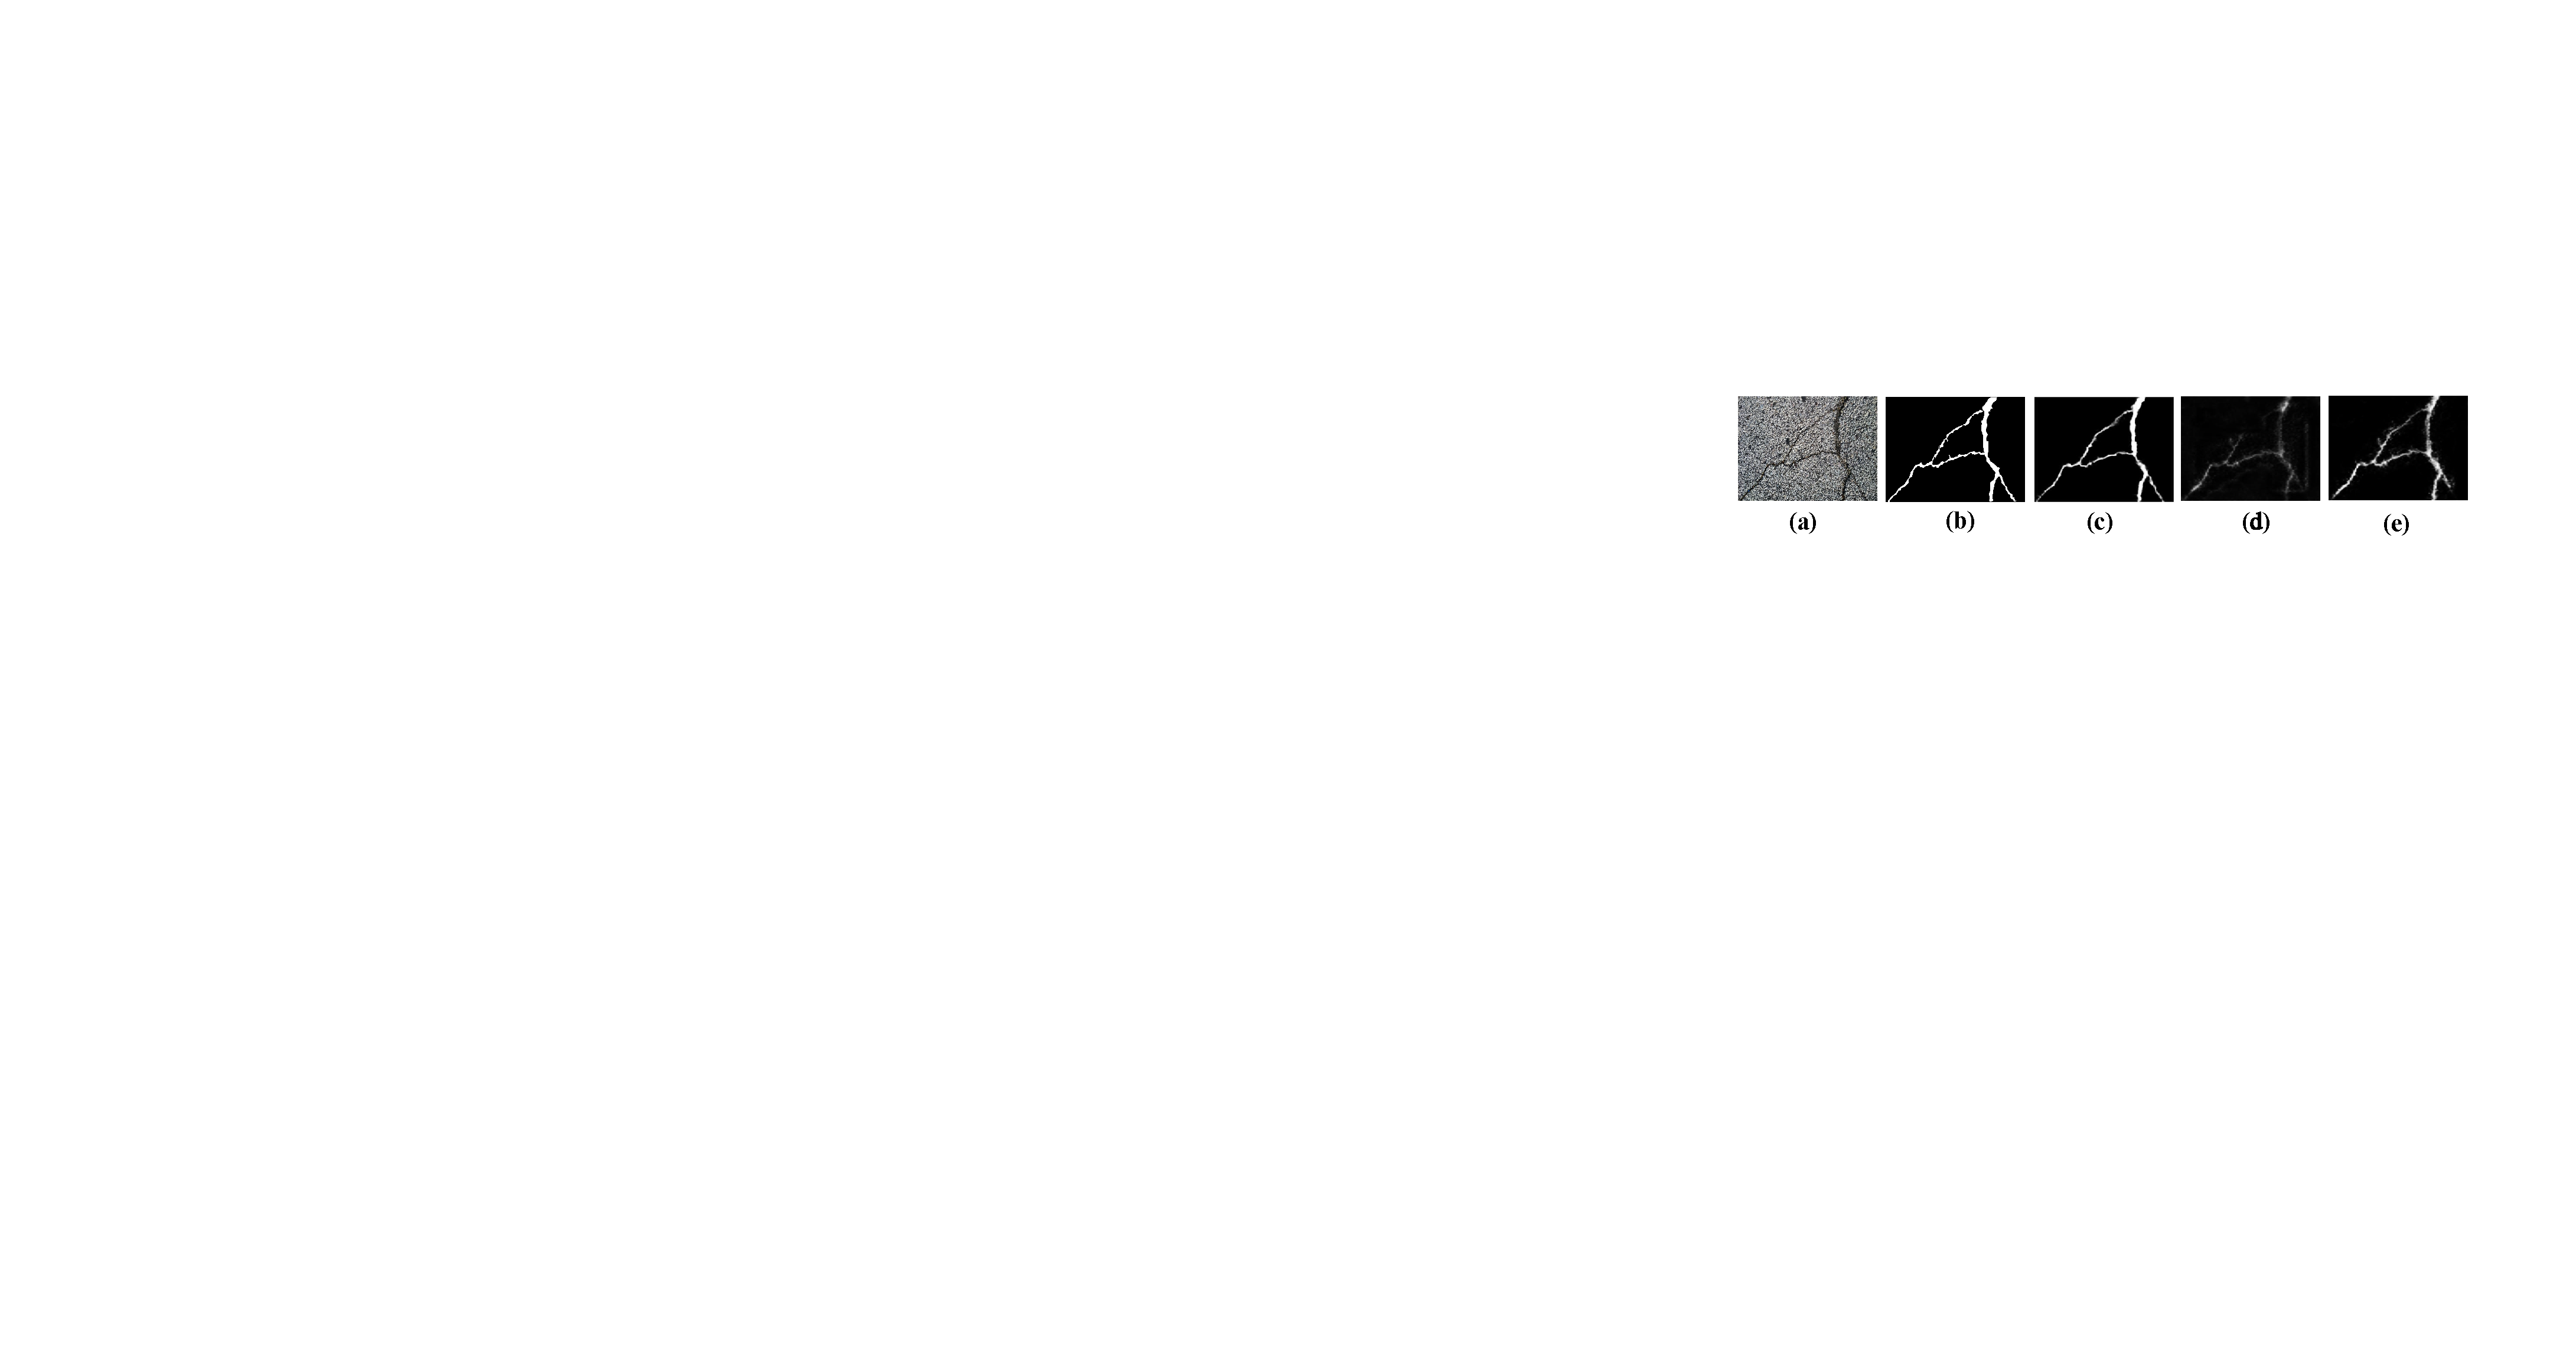
\includegraphics[width=0.85\linewidth]{abl1019.pdf}
\caption{\textcolor{red}{Qualitative comparison of three FAM configurations in Table~II on a purposefully selected
illustrative case from the Crack500 test set.
(a) Input. (b) Ground truth.
(c) Prediction of \emph{Baseline + FAM (Full)}, which fuses the high- and low-frequency branches; per-image AIU $=$ 0.63.
(d) Prediction of \emph{Baseline + FAM (High-Freq)}; per-image AIU $=$ 0.46.
(e) Prediction of \emph{Baseline + FAM (Low-Freq)}; per-image AIU $=$ 0.42.
This illustrative example qualitatively shows the complementary behavior of the two frequency branches; dataset-level conclusions are based on Table~II.}}
\label{ablavis_rebuttal}
\end{figure}

\textcolor{red}{In addition, the following sentence has been added to Section~IV-F (Qualitative Results) to state the
selection criteria of the method-comparison figure (Fig.~5):}

\textcolor{red}{
The examples in Fig.~5 are purposefully selected illustrative cases from the five test sets.
They cover thin hairline cracks, coarse pavement texture, shadows and uneven illumination, and crack-like
distractors; they are not random or best-performing samples, and all methods are compared on identical inputs.
}\\[10pt]

%%%%%%%%%%%%%%%%%%  end R1-Q1  %%%%%%%%%%%%%%%%%%%%%%%%


%%%%%%%%%%%%%%%%%%  R1-Q2  %%%%%%%%%%%%%%%%%%%%%%%%
{\color{BlueGreen} \textbf{Q2 Comments to the Author:}

\textbf{The overall descriptions of FAM, T-M, and HFM---particularly in Sections III-B and III-C---remain verbose and
would benefit from a clearer separation between intuition and formalism. Providing a concise, high-level explanation
of each module's purpose before introducing the mathematical expressions would significantly improve readability and
help interdisciplinary readers better understand the design motivations.}}

\textbf{Response:}
We thank the reviewer for this insightful suggestion, which has significantly improved the readability of the method
section. In the revised manuscript, Sections~III-B and III-C have been restructured following exactly the principle
suggested by the reviewer, namely a clear separation between intuition and formalism:

\begin{enumerate}
    \item \textbf{Intuition first.} Each of the three modules (FAM, T-M, and HFM) now begins with a concise
    ``\emph{Design intuition}'' paragraph that explains, in plain language and without any equation, what problem the
    module solves and why it is designed this way.

    \item \textbf{Formalism afterwards, condensed.} The mathematical formulation follows the intuition paragraph.
    The previously scattered equation-by-equation commentary (several separate explanatory passages inserted after
    Eqs.~(1)--(4) in the last revision) has been consolidated into brief remarks, and overlapping explanations of the
    FAM mechanism, which appeared three times in slightly different wording, have been merged into a single passage.
    As a result, Sections~III-B and III-C are now \emph{shorter} than in the previous version while conveying the
    same technical content.
\end{enumerate}

\textcolor{red}{In the revised manuscript, the newly added ``Design intuition'' paragraphs are shown below:}

\textcolor{red}{
\textbf{(Section~III-B, before the formulation of FAM)}
\textbf{Design intuition of FAM.} Road cracks appear as sparse and sharp intensity discontinuities embedded in slowly
varying pavement context. In the feature space, the former concentrates in the high-frequency band, whereas the
latter dominates the low-frequency band. The FAM is therefore designed to (i) decompose each backbone feature into a
high-frequency and a low-frequency component, (ii) let the two components exchange complementary information, so that
edge responses acquire contextual support and contour responses are cleansed of texture noise, and (iii) re-weight and merge the two bands using learnable weights. The output is a frequency-balanced feature in which crack
evidence is amplified relative to background texture. The remainder of this subsection formalizes these three
steps.
}

\textcolor{red}{
\textbf{(Section~III-B, before the formulation of the T-M decoder)}
\textbf{Design intuition of T-M.} The T-M decoder aggregates the frequency-aware features of the three deepest
levels: deeper features indicate \emph{where} a crack is likely to exist, while shallower ones describe its shape
more precisely. Multiplying adjacent feature maps promotes responses that are jointly activated across semantic levels, thereby suppressing level-specific noise and producing a cleaner coarse localization map $S_1$.
}

\textcolor{red}{
\textbf{(Section~III-C, before the formulation of HFM)}
\textbf{Design intuition of HFM.} The HFM addresses two questions during refinement. The first is \emph{where to
refine}: at refinement stage $i$, the current guidance map $S_i$ acts as a spatial prior that amplifies
crack-relevant regions of the deeper feature. The second is \emph{what to keep}: a cross-layer feature interaction between
adjacent layers determines which high-resolution details are consistent with this prior and should be preserved.
These operations refine accuracy with a moderate throughput cost, as quantified in Table~II. The following
formulation details the two steps.
}

In addition, the redundant explanatory passages of the previous round have been merged and condensed (the removed
redundancies are not marked in red, to keep the marking readable). We believe the method section is now
significantly easier to follow, especially for interdisciplinary readers.\\[10pt]

%%%%%%%%%%%%%%%%%%  end R1-Q2  %%%%%%%%%%%%%%%%%%%%%%%%


%%%%%%%%%%%%%%%%%%  R1-Q3  %%%%%%%%%%%%%%%%%%%%%%%%
{\color{BlueGreen} \textbf{Q3 Comments to the Author:}

\textbf{The paper would benefit from a short subsection discussing typical failure cases or limitations. Presenting a
small number of representative failure examples and briefly analyzing why FANet struggles in those conditions would
provide a more balanced understanding of the model's behavior and practical boundary conditions.}}

\textbf{Response:}
We thank the reviewer for this constructive suggestion, which makes the experimental analysis more balanced.
In the revised manuscript, we have added a new subsection, \textbf{``Failure Cases and Limitations''
 (Section~IV-H)}, placed after the ablation studies. It presents selected failure examples from FANet's own
predictions, grouped into two observed failure modes, analyzes
the underlying reasons within the frequency-aware design, and summarizes the practical boundary conditions and future
directions of FANet.

\textcolor{red}{In the revised manuscript, the newly added subsection is shown below (figure numbers in the quoted text refer to the revised manuscript, where the failure-case figure is Fig.~7; it is reproduced below):}

\textcolor{red}{
\textbf{IV-H. Failure Cases and Limitations.}
Although FANet achieves the highest values among the methods compared in Table~I, it still struggles under two identifiable
conditions. Fig.~7 shows two illustrative failure cases selected from the test sets. In each column, the top row is the input
image, the middle row is the ground truth, and the bottom row is our prediction, so that the gap between the ground
truth and our result can be read directly.
}

\textcolor{red}{
\textbf{(1) Fragmentation of low-contrast cracks.} When the local contrast between a crack and the surrounding pavement is weak, some crack segments receive low prediction confidence. As shown in Fig.~7(a), the ground-truth crack forms a continuous structure, whereas the prediction exhibits weak and uneven responses along the crack, so that several portions are barely activated and the predicted crack loses continuity.
}

\textcolor{red}{
\textbf{(2) Under-segmentation of fine hairline cracks.} When cracks are only a few pixels wide, their responses can be weak relative to the surrounding pavement texture. As shown in Fig.~7(b), the main crack is recovered, but several fine branches visible in the ground truth are missed or only partially detected.
}

\textcolor{red}{
These observations suggest that the current design is least reliable when crack evidence is not a sufficiently
distinct sparse high-frequency signal, particularly at very low contrast or very small width. In addition, two
limitations are worth noting. First, the two-step coarse-to-fine pipeline reduces throughput by 22.7\% (from 13.2 FPS for the PVT
baseline to 10.2 FPS for the complete model) on the same hardware, as reported in Table~II. Second, FANet is
trained with binary cross-entropy only and imposes no explicit topological continuity constraint, which may contribute
to the fragmented predictions above. We plan to explore topology-aware objectives, contrast-adaptive frequency
weighting, and complementary sensing modalities such as depth or infrared imaging to push these boundaries in future
work.
}

\begin{figure}[H]
\centering
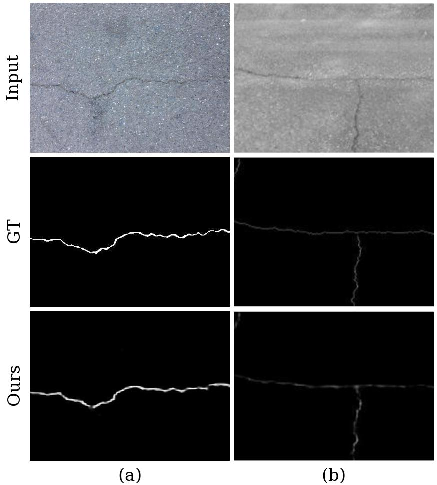
\includegraphics[width=0.62\linewidth]{failure_cases_v4.pdf}
\caption{\textcolor{red}{Illustrative failure cases of FANet. In each column, the top, middle, and bottom rows show the input image, the ground truth, and our prediction, respectively. (a) A low-contrast crack whose continuous ground-truth structure is only weakly and unevenly recovered, losing continuity at several locations. (b) A fine hairline crack whose main structure is recovered while several fine branches are missed or only partially detected.}}
\label{failure_rebuttal}
\end{figure}

\vspace{6pt}

%%%%%%%%%%%%%%%%%%  end R1-Q3  %%%%%%%%%%%%%%%%%%%%%%%%

%%%%%%%%%%%%%%%%%%%%%%%%%%%%%%%%%%%%%%%%%%%%%%%%%%%%%%%%%%%%%%%%%%%%%%%%
\section{Response to Reviewer 2}
%%%%%%%%%%%%%%%%%%%%%%%%%%%%%%%%%%%%%%%%%%%%%%%%%%%%%%%%%%%%%%%%%%%%%%%%

{\color{BlueGreen} \textbf{Comments to the Author:}

\textbf{The authors have addressed all my concerns. I recommend acceptance. Thanks.}}

\textbf{Response:}
We sincerely thank the reviewer for the positive evaluation of our revised manuscript and for recommending
acceptance. The reviewer's constructive comments in the previous round have contributed greatly to improving the
quality of this work.\\[10pt]

\clearpage

{\small
\bibliographystyle{IEEEtran}
\bibliography{IEEEfull}
}

\end{document}
